\chapter{Radiance}
\label{ch:radiance}

\begin{center}
\begin{minipage}{\textwidth - 2em}
\itshape\small
An extract from~\cite{nicodemus63}, introducing the formal definition of
radiance. The excerpt has been retypeset, the symbols designating the various
quantities brought in line with current practice, \gls{si} units substituted and
references adapted to the typographic style of this document.
\end{minipage}
\end{center}

\begin{center}
\textit{\Large American Journal of Physics, Vol. 31, pg. 368--377, 1963}

%{\Large \adfopenflourishleft\adfopenflourishright}\\
{\Large \adfflourishleftdouble\quad\adfast9\quad\adfflourishrightdouble}\\

\textsc{Fred E. Nicodemus}
\vspace{3pt}

\textit{\small Sylvania Electronic Systems\\
West, Electronic Defense Laboratories, Mountain View, California}

\vspace{3pt}
(Received 22 October 1963)

{\Large \adfclosedflourishleft\quad\adfclosedflourishright}\\

\textsc{Abstract}

\vspace{6pt}
\begin{minipage}{.786\textwidth}
%\hrule\vspace{3pt}
\small
Wide generality for optical radiometry can be achieved by treating the basic radiometric
quantities as field quantities. The treatment is that of classical ray optics,
with
emphasis on the geometrical relations involved. It is shown that radiance,
defined as
\begin{displaymath}
L_e \equiv \frac{\partial^2 \Phi_e}{\partial\omega \; \cos\theta\partial A}
\qquad \left[\si{\watt\per\square\meter\per\steradian}\right],
\end{displaymath}
the radiant flux or power per unit solid-angle-in-the-direction-of-a-ray per
unit
projected-area-perpendicular-to-the-ray, has the same value at any point along this ray
within an isotropic medium, in the absence of losses by absorption, scattering, or
reflection. More generally, the quantity $L/n^2$ (where $n$ is the index of
refraction of
the medium) in the direction of a ray is shown to be invariant along that ray,
even across
a smooth boundary between different lossless media. The usefulness of this
invariant
property of radiance is illustrated by examples of practical applications.
%\vspace{3pt}\hrule
\end{minipage}
\end{center}

\section{Introduction}

Why does a photographic exposure meter give the same reading over a wide range
of distances from a uniformly illuminated blank wall with a rough, weathered surface?
Of course the indication changes when it is held so close to the wall that its
shadow,
or that of the supporting arm and hand, reduces the illumination, or when it is
held
so far away that radiation is also received from the surrounding background beyond
the edges of the wall. But between these extremes, the indication will remain
constant.
Nor is it possible with an external lens, however large or “fast,” to focus more radiant
power from the wall onto the exposure meter to obtain a higher reading.

Why does a spectroscopist obtain maximum energy with the following procedure?
Focus an image of the source onto the entrance slit of the spectroscope.
Arrange the source and focusing optics so that the image is just large enough
to fill the slit completely (if the source is not uniform, the slit must be
filled by the brightest uniform region of the image), and so that the
rays which cross to form the image diverge widely enough after passing through
the slit that they completely fill the collimating optics of the
spectroscope. Once this condition has been achieved, it is useless to attempt
to focus more radiant power through the instrument from the same source.

If it is given that the earth's surface radiates a total (in all directions) of
$w\si{\watt\per\square\meter}$, how can we quickly estimate the irradiance
$E_e$,
in $\si{\watt\per\square\meter}$ due to this source alone without atmospheric
attenuation, at a horizontal receiving surface carried on an earth satellite
vehicle?
For simplicity, assume that the earth is a perfectly diffuse radiator.

These situations all involve extended sources of radiation. It has been my experience
that most people find it peculiarly difficult to master the fundamental concepts and
relations of radiometry (or photometry) as they apply to extended sources. And I
have
come to believe that the key to this difficulty lies in the interrelated concepts of an
elementary beam of radiation and its radiance (or luminance).

A brief definition of radiance is given in the abstract and is discussed in more
detail
directly. It is helpful to note here that radiance is analogous to the familiar property
of visual brightness, or more exactly to the photometric quantity luminance.
Also for convenience, Table~\ref{tab:radiophoto}\footnote{[Table~I in the
original---\textit{Ed.}]}
lists the radiometric quantities, symbols, and units used in this paper.

Sometimes radiance is defined as applying only to sources of radiation
(see \citerad{kelton1963infrared}\footnote{[Cited in the original as ``Report of
WGIRB (Working Group on Infrared Backgrounds)---Infrared Target and Background
Radiometric Measurements---Concepts, Units, and Techniques'', Report 2389-64-T,
NAVEXOS P-2406 (IRIA, Institute of Science and Technology, University of
Michigan, Ann Arbor, Michigan, January 1962), pp. 3-4 Contract No. Nonr-1224(12)
---\textit{Ed.}]}, \citerad{bell59}\footnote{Essentially the same
material also appears as “Report of the Working Group on Infrared Backgrounds;
Part II: Concepts and Units for the Presentation of Infrared Background
information,” Report No. 2389-3-5 (Engineering Research Institute, University of
Michigan, Ann Arbor, Michigan, November 1956), Contract No. Nonr-1224 (12)}
and~\citerad{jenkins50}). Frequently it is applied also to images of a source,
and it is shown that, in the absence of attenuation, the radiance (or luminance)
of an image is equal to that of the source in the direction of any ray reaching
it from the source (see~\citerad{jenkins50}).

The usefulness of defining radiance more broadly as a field quantity which can
be evaluated at any point along a ray is also pointed out, particularly with
reference to diffuse sources such as a volume of emitting gas
(see~\citerad{kelton1963infrared}).
It is established that radiance has the same value everywhere and in all
directions, within an isotropic region in thermal equilibrium
(see~\citerad[p.~183--196]{planck57} and~\citerad{richtmyer47}).
However, I have not found anywhere a completely general treatment of invariant
property of radiance, defined as a field quantity, although such a treatment can
greatly simplify the understanding of many radiometric situations, as well as
the computation or estimation of the amount of radiant power or flux incident on
a receiver or detector, or passing through some aperture of interest, in a wide
variety of circumstances. None of the material presented here is new, rather it
is implicit in many publications, but it is not explicitly in any that I am
aware of.

For generality, we define radiance as a field quantity which can be evaluated at
any point on any surface through which radiant power or flux is passing.
This includes, but is not restricted to, the surfaces of a source, a receiver,
or any intermediate optical element such as a mirror, lens, or stop (aperture
limiting a beam of radiation). On this basis, radiance is defined as the radiant
flux or power per unit solid-angle-in-the-direction-of-a-ray per unit
projected-area-perpendicular-to-the-ray.
More precisely, in a given direction from a point on a surface through which radiant
energy is passing,

\begin{equation}\label{eqn:nicodemus1}
L_e \equiv \frac{\partial^2 \Phi_e}{\partial\omega \; \cos\theta\partial A}
\qquad \left[\si{\watt\per\square\meter\per\steradian}\right],
\end{equation}
where $L_e = $ the radiance at that point in the given direction,
$\Phi_e = $ the radiant flux or power flowing through the surface
(within the solid angle $\omega$ and the area $A$) $[\si{\watt}]$,
$\omega = $ the solid angle filled by the rays along which the
radiation is propagated (including, of course, the ray extending
in the given direction through the given point of the surface)
$[\si{\steradian}]$,
$A =$ the area of the surface (including, of course, the given point)
$[\si{\square\meter}]$, and $\theta = $ the angle between the given direction
and the normal to the surface at the given point $[\langle dimensionless
\rangle]$.
We return to this definition later as the basic radiometric quantities are
presented in a logical sequence leading up to the proof of the invariance
property. It is shown that the value of $L$ in the direction of any ray
has the same value at all points along that ray within an isotropic medium,
in the absence of losses by absorption, scattering, or reflection.
More generally, the quantity $L/n^2$ (where $n$ is the index of refraction of
the medium) in the direction of a ray is shown to be invariant along that ray,
even
%page 371
across a smooth non-reflecting boundary between different lossless media.
The treatment of real situations, where absorption, scattering, and reflection
can not be neglected, is also discussed.

\section{Analysis}

We define a radiation field as a region in which radiant power is propagated,
at a velocity characteristic of the region or medium and independent of
direction,
along straight non-interfering rays which may pass in any direction through
any point within the region. The radiant power or flux may vary with position
and direction, but only in a continuous manner, so that a finite amount of power
can flow only through a finite area and a finite solid angle. Thus, here and in
actuality, there is no such thing as a point source, with all of the power
traveling along rays which intersect at a single mathematical point; nor is
there such a thing as a perfectly collimated beam with all of the power
traveling along rays which are perfectly parallel\footnote{\label{note:nicodemus6}
The assumptions involved here are discussed with greater rigor by Planck. It can
be shown that his analysis does not conflict with the results presented here,
although there are apparent differences due to the very different terminology
and symbols used. See~\citerad[pp.~173--177]{planck57}}.

\begin{figure}
\begin{center}
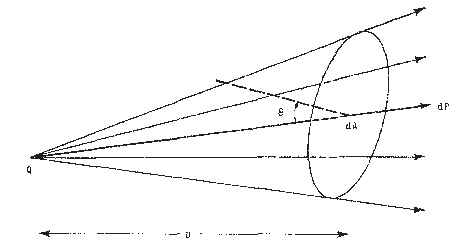
\includegraphics{figures/nicodemus1963-fig1.pdf}
\end{center}
\caption{An elementary pencil of radiation}
\label{fig:nicodemus1}
\end{figure}

In order to analyze this situation, let us first consider only the distribution
of power flow as a function of direction. We define an elementary pencil of rays
through a point $Q$ as including all of the rays which pass from $Q$ through an
element of area $dA$ at a distance $D$ from $Q$ which is very large in relation
to
the linear dimensions of $dA$ (see Figure~\ref{fig:nicodemus1}).
The solid angle subtended at $Q$ by $dA$ is given by
\begin{equation*}
\d\omega = \frac{\cos\theta \d A}{D^2}
\qquad \left[\si{\steradian}\right],
\end{equation*}
where $\theta$ is the angle between the normal to $dA$ and the pencil of rays,
i.e., $\cos\theta\cdot dA$, is the projected area of $dA$ normal to this pencil.
If we next consider $Q$ not as a mathematical point, but as having dimensions
which, however, are very small compared to the dimensions of $dA$ (and, hence,
extremely small compared to $D$), the power which flows along the rays in this
pencil from $Q$ to $dA$ can be expressed as
\begin{equation*}
\d\Phi_e = I_e \d\omega = I_e \frac{\cos\theta \d A}{D^2}
\qquad \left[\si{\watt}\right],
\end{equation*}
where
\begin{equation}
I_e \equiv \frac{\partial \Phi_e}{\partial \omega}
\qquad \left[\si{\watt\per\steradian}\right]
\end{equation}
is defined as the \textsl{radiant intensity} (see Table~\ref{tab:radiophoto}) of
$Q$ as a “point” source of radiation (e.g., a virtual source, such as the image
of an illuminated pin hole) \emph{in the direction of the pencil} (the direction of
$dA$ from $Q$). Note that $I_e$ may vary with direction and is a constant only
for an isotropic source. In general, the power received from a distant “point"
source is given by
\begin{equation}
\Phi_e = \int I_e \d\omega
\qquad \left[\si{\watt}\right],
\end{equation}
where the integration is carried out over the entire solid angle subtended at
the source by the receiver.

For completeness, we also look briefly at the purely spatial variation, although
this quantity is more easily understood and is not so often a source of
difficulty
or misunderstanding. If we consider an element of surface $dA$, situated
anywhere
in a radiation field, the total amount of radiant power passing through it
(either
into it from a hemisphere, or out of it into a hemisphere) can be expressed as
\begin{equation*}
\d\Phi_e = E_e \d A \quad \textrm{or} \quad \d\Phi_e = M_e \d A
\qquad \left[\si{\watt}\right],
\end{equation*}
where
\begin{equation}\label{eqn:nicodemus4}
E_e \equiv \frac{\partial \Phi_e}{\partial A}
\qquad \left[\si{\watt\per\square\meter}\right]
\end{equation}
is the \textsl{irradiance} (see Table~\ref{tab:radiophoto}), the surface density
of radiant power flowing into the surface at a point from a complete hemisphere
(or, sometimes, from a stated solid angle which is less than a hemisphere), and
where
\begin{equation}\label{eqn:nicodemus5}
M_e \equiv \frac{\partial \Phi_e}{\partial A}
\qquad \left[\si{\watt\per\square\meter}\right]
\end{equation}
%page 372
is the \textsl{radiant emittance} (see Table~\ref{tab:radiophoto}), the surface
density of radiant power flowing out of the surface at a point into a complete
hemisphere. Both of these quantities may vary from point to point over an
extended
surface, so that the total radiant power flowing into the surface of a receiver
is given by
\begin{equation}
\Phi_e = \int E_e \d A
\qquad \left[\si{\watt}\right],
\end{equation}
and that flowing out of the surface of a source is given by
\begin{equation}
\Phi_e = \int M_e \d A
\qquad \left[\si{\watt}\right],
\end{equation}
where the integration is carried out over the entire surface of interest in each case.

\begin{figure}
\begin{center}
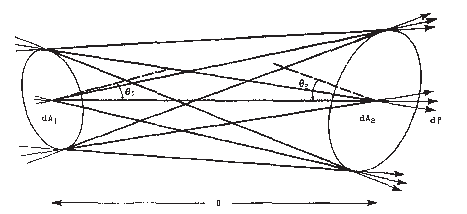
\includegraphics{figures/nicodemus1963-fig2.pdf}
\end{center}
\caption{An elementary beam of radiation between two surface elements $\d A_1$ and $\d A_2$}
\label{fig:nicodemus2}
\end{figure}

We now consider the simultaneous distribution of radiant flux in both space
and direction by examining an elementary beam of radiation. The elementary beam
of radiation between two elements of area $\d A_1$ and $\d A_2$, situated anywhere in
a radiation field where they are separated by a distance $D$ which is very large
compared to the linear dimensions of either element of area, is defined as
including
all of the rays which pass from $\d A_1$ to $\d A_2$ (or from $\d A_2$ to $\d A_1$, since either
may be the source and the other the receiver).
By inspection of Figure~\ref{fig:nicodemus2}, it can be seen that the cross
section of
the beam at either end is determined by the projected area of the element at
that end,
i.e., by $\cos\theta_1 \d A_1$ and $\cos\theta_2 \d A_2$, respectively. Also, the
solid angle
subtended at the opposite end by each element is equal to this projected area
divided by
$D^2$ in each case, giving
\begin{equation*}
\d \omega_1 = \frac{\cos\theta_1 \d A_1}{D^2}
\qquad \left[\si{\steradian}\right]
\end{equation*}
and
\begin{equation}
\d \omega_2 = \frac{\cos\theta_2 \d A_2}{D^2}
\qquad \left[\si{\steradian}\right].
\end{equation}

If we compute the projected-area-solid-angle-product (which has also been
referred
to as the ``throughput''\footnote{\label{note:nicodemus7} The term
``throughput'' appears
in the instruction manual issued by Block Associates, Inc., for an
interferometer
spectrometer. It is not known who originated the term or the precise way in
which
he would define it, but it appears to agree with the way in which it is used
here})
at each end we have
\begin{align*}
\d G_1 &= \cos\theta_1 \d A_1 \d \omega_2 = \cos\theta_1 \d A_1 \frac{\cos\theta_2
\d A_2}{D^2} \\
\d G_2 &= \cos\theta_2 \d A_2 \d \omega_1 = \cos\theta_2 \d A_2 \frac{\cos\theta_1
\d A_1}{D^2}
\end{align*}
But
\begin{equation}
\d G_1 = \d G_2 = \d G
\qquad \left[\si{\square\meter\steradian}\right].
\end{equation}

Next, let us recall the definition of \textsl{radiance}, the power per unit
projected
area per unit solid angle at a point and in a particular direction, as
\begin{equation*}
L_e \equiv \frac{\partial^2 \Phi_e}{\partial\omega\;\cos\theta \partial A}
\qquad \left[\si{\watt\per\square\meter\per\steradian}\right].
\end{equation*}

If the radiance at $\d A_1$ is $L_{e1}$ and that at $\d A_2$ is $L_{e2}$, the power
flowing
through each surface element is given, respectively, by
\begin{align}
\d \Phi_{e1} &= L_{e1} \cos\theta_1 \d A_1 d\omega_2 = L_{e1} \d G \nonumber\\
\d \Phi_{e2} &= L_{e2} \cos\theta_2 \d A_2 d\omega_1 = L_{e2} \d G.
\end{align}

But the same power is flowing through both of the surface elements that define
the
beam, since all rays through one also pass through the other and energy is
conserved
(we have postulated no loss), so
\begin{equation}
\d \Phi_{e1} = \d \Phi_{e2}\quad \textrm{and} \quad L_{e1} = L_{e2} = L_e.
\end{equation}

Since the choice of $\d A_1$ and $\d A_2$ is quite arbitrary, and they can define a
beam between any widely separated points along a particular ray, it follows that
\emph{the value of $L_e$ in the direction of a ray must be invariant along that
ray within an isotropic medium}.
The value of $L_e$ at any point will vary with direction, and the value of $L_e$
for rays from a particular direction (parallel rays) will vary with position on
any surface which they intersect. Hence, in general, the flux passing through a
given surface and within a given solid
%page 373
angle is given by
\begin{equation}\label{eqn:nicodemus12}
\Phi_e = \int \int L_e \cos\theta \d A \, \d \omega
\qquad \left[\si{\watt}\right],
\end{equation}
where the integration is carried out over the entire surface (with respect to
the projected area perpendicular to any given direction) and over all directions
included within the given solid angle.

\begin{figure}
\begin{center}
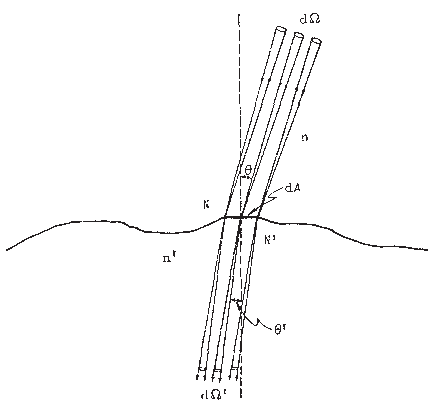
\includegraphics{figures/nicodemus1963-fig3.pdf}	
\end{center}
\caption{Refraction at a smooth boundary between media of
different refractive indices ($n$ and $n'$)}
\label{fig:nicodemus3}
\end{figure}

In order to generalize still further, we examine the situation where a beam of
radiation passes through a smooth surface separating two media with different
refractive indices (see Figure~\ref{fig:nicodemus3}). The power incident on any
surface element $\d A$ through any element of solid angle $\d \omega$ in the first
medium and that from the same beam emerging from the same surface element into
a solid angle $\d \omega'$ in the second medium must be the same, if there are no
losses by reflection, absorption, or scattering (we are still concerned purely
with ray geometry and defer questions of Fresnel reflection losses, etc., until
later). This power is given by
\begin{equation}\label{eqn:nicodemus13}
d\Phi_e = L_e\,\cos\theta \d A\, \d \omega = L_e'\,\cos\theta' \d A\, \d \omega'
\qquad \left[\si{\watt}\right].
\end{equation}

By Snell's law of refraction, we write
\begin{align}
n\sin\theta &= n' \sin \theta' \\
\therefore\quad n\cos\theta \d \theta &= n' \cos\theta' \d \theta'.
\end{align}
Also,
\begin{equation}
\d\omega = \sin\theta\d\theta \d\phi
\quad \textrm{and} \quad
\d\omega' = \sin\theta'\d\theta' \d\phi
\end{equation}
(the azimuth angle $\phi$ of a ray is not changed by refraction). Hence,
\begin{equation*}
\frac{L_e \d A \cos\theta \d\omega}{L_e' \d A \cos\theta' \d\omega'} =
\frac{L_e \cos\theta \sin\theta \d\theta \d\phi}{L_e' \cos\theta' \sin\theta' \d\theta' \d\phi}
\frac{L_e n'^2}{L_e' n^2} = 1
\end{equation*}
\begin{equation}
\therefore\quad \frac{L_e}{n^2} = \frac{L_e'}{n'^2} \label{eqn:nicodemus17}
\end{equation}
Thus, \emph{the quantity $L / n^2$ in the direction of a ray is invariant along
that ray}, even as it passes through a smooth boundary surface between media of
different refractive indices, if there are no losses by reflection, absorption,
or scattering (see~\citerad[pp.
266--268]{martin60}\footnote{\label{note:nicodemus8__}Martin's proof is given
only for the luminance $L_v$ of an image, but with
only slight modification it, too, is easily generalized to apply to any
point along a ray.}). It is also apparent from Equation~\ref{eqn:nicodemus17}
that the value of $L_e$ in the direction of a ray will be the same at any
point along such a ray which lies in a medium with the same index, regardless
of passage through other media, such as refractive lenses, at intermediate
points.
Total reflection from a smooth surface merely changes the direction of a
beam and does not alter $L_e$. This can be verified in detail by an analysis
similar to that just given for refraction at a smooth boundary.

A “smooth” surface, as the term is used here, is defined to include any
surface where it is possible everywhere to construct a tangent plane,
i.e., where every surface element can be treated as common to the
surface and to a plane tangent to the surface at that point.

It should be recognized, of course, that all real situations involve
some losses by absorption, scattering, or reflection, although it is
frequently possible to keep the losses to negligible amounts
by careful design. Also, in real situations we are concerned with sources
and receivers, not hypothetical elements of surface.

In the foregoing analysis, we have attempted to achieve as much generality
as possible by considering radiation fields and surface elements placed in
those fields with as few restrictions as possible. In this way, the results
of the analysis can be extended widely to describe the radiometric quantities
at the surfaces of almost any receiver of radiation in terms of those quantities
at any source, or at any intermediate location where it may be convenient to specify or measure
%page374
them. This has been done purely in terms of ray geometry, neglecting losses
by absorption, scattering, and reflection. Such losses, where they are
not negligible, can be accounted for by multiplying the radiometric quantities,
determined from ray geometry only, by the appropriate factors.
For example, if the radiance along a particular ray at a source is
$L_{es}$, and the radiant transmittance (see Table~\ref{tab:radiophoto}) along
its path (taking into account the source spectrum and the spectral transmittance
(see Table~\ref{tab:radiophoto}) of the intervening medium) from source to
receiver is $\tau$, and source and receiver both lie in the same medium (same
index of refraction), then the radiance at the receiver in the direction of
this same ray is given by $L_{er} = \tau L_{es}$. If, in addition, this same
ray has also been imperfectly reflected by a mirror at some point along its
path to the receiver, the radiance at the receiver becomes $L_{er} = \rho \tau L_{es}$,
where $\rho$ is the radiant reflectance (see Table~\ref{tab:radiophoto}) of
the mirror.

A situation of even more importance, perhaps, is the effect of reflection loss
on the radiance along a ray which is refracted at a boundary between two media
of different refractive indices.
Fresnel’s equations require that there be some reflectance at any simple
boundary between two such media. Here, if the radiance along the incident ray
is $L_e$, and if the radiant reflectance for the particular angle of incidence
is $\rho$, the radiance along the refracted ray in the second medium
will be given by
\begin{equation}
L'_e = L_e \frac{n'^2}{n^2} (1-\rho)
\qquad \left[\si{\watt\per\square\meter\per\steradian}\right].
\end{equation}
Note, however, that it may be possible to reduce $\rho$ to a negligible value,
at least for a limited range of wavelengths and angles of incidence, by the
use of so-called antireflection coatings, thus approaching the condition
described by Equation~\ref{eqn:nicodemus17}.

\section{Practical applications}
[omitted---\textit{Ed.}]

\ifomit
Before describing some situations which illus-
trate the usefulness of the invariant property of
radiance, we consider briefly the limitations
governing the application of the concepts of
radiance and radiant intensity to real sources.
To look first at the extremes, it is obviously
meaningless, with respect to a receiver at the
earth’s surface, to speak of the radiance of a star
or the radiant intensity of a clear sky. Even the
nearest star, in spite of its huge size, subtends
such a small solid angle at the earth that it
defines a pencil, rather than a beam, of radiation.
Hence it is characterized by its radiant intensity.
Conversely, the sky subtends so large a solid
angle that, for most purposes it is necessary to
recognize the variations in its radiance in differ-
ent directions from a receiver at the ground.

Most sources fall into an intermediate category
where they may be characterized by their radi-
ance or their radiant intensity, depending on the
distance of the receiver and the size of the smal-
lest solid angle or resolution element which is
considered significant. Thus a planet, like a star,
will ordinarily define a pencil of radiation, i.e.,
its radiant intensity is the quantity of importance
in determining the total radiant power reaching
the aperture of a telescope on earth from the
entire planet. However, the amount of radiant
power in various portions of a highly magnified
image of the planet Mars, for example, is a func-
tion of the radiance of the corresponding portions
of the planet's surface in the direction of the
earth. Similarly, the plume of a large missile in
powered flight is clearly an extended source, with
a complicated spatial distribution of varying
radiance, with respect to a receiver at a distance
of a few hundred feet. However, from high alti-
tudes such a plume may be treated as a point
source, characterized by its radiant intensity in

FIG. 4. A simple radiom-
eter; A sensitive receiv-
er (detector) of area a
is located at one end of
an opaque tube of length
6 with an aperture of area
A in the opposite end of
the tube to limit the beam
of rays incident upon the
receiver.

% end of page

the direction of a detection device on the ground
in most i11sta11ces where the field of View of the
device is large enough to permit acquisition and
tracking of the moving target without unusually
complex and expensive equipment.
The 'L1sefu111ess of the invariant property of
radiance can be illustrated in connection with a
very simple radiometer consisting of a detector
with a flat sensitive surface of area a, such as a
common lead sulphide cell, mounted in a tube of
length 4?, with a limiting aperture of area at the
tar end to define the beam of radiation incident
on the detector (see Fig. 4). It is assumed that
the ratio of /5 to the linear dimensions of the
detector is large enough so that, to the desired
degree of accuracy, the detector subtends the
same solid angle Qza/£3 at all points of the
entrance aperture. It such an instrument is
placed close enough to an extended source of
uniform radiance _N, the total radiant power"
incident on the cell (measured by its electrical
response) can be written immediately as

P 2 rA7,in 3 viva a/.52 [W],

where T is the total radiant transmittance over
the path from source to cell. This is possible
because We know that, in the absence of loss, the
radiance along each ray at the entrance aperture
is N, the same as at the source along the same
rays. And at this position the rays fill an area A
and a solid angle Q=a/W at each point Within
that areal In practice, by measuring P from the
response of the cell, and knowing 7-, A, a, and -E,
we can compute the radiance of an unknown
imzform source as

P59
N z
7-A at

(19)

UN - c111‘? - sr‘l:]. (20)

ll 7 is unlrnovvn, as is frequently the case for
atmospheric transmittance, we will measure in-
stead the apparent radiance (at the radiometer)

Pr?
N’ 2 izrv rm

[VV ~ cm“? - sr‘1].
Au,

(21)

Probably, in a practical situation, the values of
ill, :1, and -ti, will not be determined individually.
Instead, the factor

rainzirra,/ezupd,/‘N’=Pft.iil’nv [Cassi] (22)

3 riELD srse
m-**“ j; (In rocit

Lriis inn PMNE)

APERTURE STU?

FIG. 5. Nearusmall-source (Jones method) calibration.
Source completely Within region bounded by XZ and YZ,
which make an angle 6 with the optical axis. 6=ha.lf-field
angle. P=arbit.rary point of source. Rays from any such
point P Within a cone of half-angle 8 will uniformly irradiate
the field stop as shown.

which has been called the “throughput,” will be
determined by a calibration measurement of a
source of known radiance at a distance Where 7
is known or is practically unity (negligible
attenuation).
Another illustration of useful application of
the general property of invariance, at points
Where rays do not cross to form an image of the
source, is in connection with the so-called Jones
Wethodg =10 for calibrating a radiometer. As shown
in Fig. 5, a small source (area small compared
with the area of the radiometer aperture) is
placed close to the radiometer Where it will uni-
formly irradiate the field stop of the instrument.
In order to do this, the source must be small
enough and close enough so that the radiometer
aperture subtends, at every point of the source,
an angle greater than the field angle of the in-
strument. As can be seen in Fig. 5, this means
that the source must lie entirely Within the region
enclosed by the cone represented by the lines
XZ and YZ, which meet at Z to form an angle
equal to the field angle of the radiometer, as
shown.
In the following approximate treatment, it is
assumed that the optics are ideal, so that a
parallel bundle of rays incident on the aperture
stop of the instrument is sharply focused at a

9 This method was first used by Dr. R. C. Jones in the
fall of 1951 on Navy Contract NObsr 42179. The method
became known by word of mouth, and was first described
in writing in “An Unusual Method for Calibrating an
Infrared Radiometer” (Polaroid Corporation, 19 Septem~
ber 1955, Memorandum 614) under Navy Contract
NOhsr 63175.
1° “The Jones Method of Radiometer Calibration” Tech»
mignes (Barnes Engineering Company, winter, 1957).
Reprints of this article have also been issued as Barnes
Engineering Infrared

% end of page

376

APERTURE

FIELD

FIG. 6. Alternative illustration of Jones method of calibra-
tion. P’ is an arbitrary point within the field stop.

single point lying in the field stop. Also, it is
assumed that the field angle is small so that for
the angle 0 shown in Fig. 5, coso'- 1.

Consider any point P on the radiating surface
of the source. It is apparent in Fig. 5 that the
rays emitted from P within a solid angle 9 equal
to the field angle of the radiometer will uniformly
irradiate the field stop. If the radiance of the
source is N5, and its projected area (normal to
the optic axis) is As, the total radiant power thus
radiated from all points of the source through the
field stop (in the absence of absorption, reflection,
and scattering losses) is given by

P = N.A.rz [W]. (23)

Alternatively, as illustrated in Fig. 6, we may
consider any point P’ within the field stop. All
rays reaching P’ from the source must travel
parallel to each other in a single direction from
the source to the radiometer aperture. There they
will fill an area of the aperture equal to AS, the
projected area of the source. They are then
focused onto P’. The effective aperture area As
subtends a solid angle at P’ given by

[Sr].

where F is the focal length of the radiometer
optics. Since the radiance at the field stop in the
direction of any of the rays from the source is
equal to the source radiance N3, we can write

[W].

where A F is the area of the field stop. Since the
field solid angle is given by

w%As/F2 (24)

P=N.A ,.~o.»=NsA FA./F2 (25)

s2=A F/F2 [Sr], (26)

FRED E. NICODEMUS

it can be seen that
P:-N..A_.A F/F2=N.A,S2 [W], (27)

in agreement with Eq. (23). Note that in this
case the source is not imaged at the field stop
where the value of radiant power P is being
evaluated.
\fi

\section{Discussion of introductory examples}

In the Introduction we described three situations involving extended sources.
It should be clear from Equation~\ref{eqn:nicodemus13} that the exposure meter must
give the same response, regardless of distance or orientation, as long as all
of the radiation entering it has the same value of radiance. If the wall
is perfectly diffuse, all of the rays from it will have the same radiance.
An external lens cannot change either the area or angle through which the
meter accepts radiation, whether it comes directly from the wall or after it
passes through the lens, and the value of radiance also cannot be changed
(except by attenuation, which is assumed negligible). In the same way, once
the full receiving area (entrance slit) and solid angle (subtended at the
slit by the collimating optics) of the spectrometer are filled with rays of
the maximum available radiance, there remains no way to increase any of these
quantities with additional lenses. In the last example, we must first determine
the radiance $L_e$ of the earth’s surface.
From Equation~\ref{eqn:nicodemus1} and Equation~\ref{eqn:nicodemus5} we can write
for a uniform plane diffuse radiator for which both $L_e$ and $M_e$ are constants:
\begin{equation*}
\Phi_e = \int M_e \d A = \int \int L_e \cos\theta \d A \d \omega
\qquad \left[\si{\watt}\right],
\end{equation*}
\begin{equation}
\therefore\quad M_e = L_e \int \cos\theta \d \omega
\qquad \left[\si{\watt\per\square\meter}\right],
\end{equation}
If we choose spherical coordinates with the $z$ axis perpendicular to the
radiating surface,
\begin{equation*}
\d \omega = \sin\theta\d\theta \d \phi
\qquad \left[\si{\steradian}\right]
\end{equation*}
and
\begin{equation}
M_e = L_e \int_{\phi = 0}^{2\pi} \int_{\theta=0}^{\frac{\pi}{2}}\cos\theta
\sin\theta\d\theta \d\phi
= L_e \left.\phi\right|_{0}^{2\pi} \left.\frac{\sin^2\theta}{2}\right|_{\theta=0}^{\frac{\pi}{2}} = \pi L_e
\qquad \left[\si{\watt\per\square\meter}\right].
\end{equation}
%page377
Similarly, from Equation~\ref{eqn:nicodemus1} and Equation~\ref{eqn:nicodemus4},
the irradiance at a plane surface due to uniform radiation of radiance $L_e$,
arriving within a cone of halfangle $\theta$, is given by
\begin{equation}
E_e = L_e \int \cos\theta \d\omega = \pi L_e \sin^2\theta
\qquad \left[\si{\watt\per\square\meter}\right].
\end{equation}
This gives the desired result for an earth of uniform radiance
$L_e = M_e / \pi$ which subtends a cone of half-angle $\theta$ at the
receiver ($E_e = M_e \sin^2\theta$).

\section{Summary}

It has been established that in any radiation field radiance is invariant along
a ray, in the direction of the ray, within an isotropic medium, and that the
quantity $L_e/n^2$ is invariant along a ray, in the direction of the ray,
across smooth boundaries between media with different refractive indices,
so that $L_e$ has the same value at all points along the ray lying in media
of the same index, regardless of passage through other media at intermediate
points. Practical applications of the usefulness of this invariant property have
been presented. They show that it facilitates the evaluation of the radiant
power
flowing through any surface where it is possible to determine the cross section
of a beam (the projected area of its intersection with the surface) and the
solid
angle from which rays are flowing through each point of that surface, if the
value
of radiance is known at any point along each of the rays. In practical optical
systems,
such surfaces are usually found at the stops (aperture stop and field stop) and
their images (e.g., the entrance and exit pupils and windows), and at the
surfaces
of sources and receivers, and their images.

Evaluation of radiant power becomes a very simple matter for a beam passing
through
a well-defined plane surface ($\theta$ is not a function of position) of area
$A$
and within a well-defined solid angle $\omega$ that is the same at all points of
the
surface (no vignetting) whenever it is possible to assume a uniform value of
radiance
$L_e$ throughout the beam. The general expression in Equation~\ref{eqn:nicodemus12} can
then be simplified as follows:
\begin{equation}
\Phi_e = \int \int L_e \cos\theta \d A \d \omega = L_e A \int \int \cos\theta
\d \omega =
L_e A \Omega^\perp
\qquad \left[\si{\watt}\right].
\end{equation}
The expression $\Omega^\perp = \int \int \cos\theta \d \omega$ has been called the
``weighted solid angle'' or ``projected solid angle''(see~\citerad{jones60}).
The area-solid-angle-product, ``optical invariant''
(see~\citerad{jones62a}\footnote{Although not flagged out, the concept of
invariance of the $A\Omega$ product is also used by R. Clark Jones in two other
papers: \citerad{jones53,jones62b}}), ``throughput''\cref{note:nicodemus7} or
``\'etendue'' (see~\citerad{connes58}\footnote{I am indebted to Dr. R. Clark
Jones for calling my attention to this reference}) can be given for the
unvignetted beam through a plane surface or aperture of area $A$ as
\begin{equation}
G = A\Omega^\perp = A \int \int \cos\theta \d \omega
\qquad \left[\si{\square\meter\steradian}\right].
\end{equation}
Furthermore, in most cases the solid angle is a circular cone of
half-vertex-angle
$\theta$, with its axis perpendicular to the plane. Then, using spherical
coordinates
with the $z$ axis perpendicular to the plane, the integration can be carried out thus:
\begin{equation}
G = A\int_{\phi = 0}^{2\pi} \int_{\theta=0}^{\theta}\cos\theta \sin\theta\d\theta \d\phi
=\pi A \sin^2\theta
\qquad \left[\si{\square\meter\steradian}\right].
\end{equation}
and
\begin{equation}
\Phi_e = L_e G = \pi L_e A \sin^2\theta
\end{equation}

\section{Acknowledgement}

In this report, the author has made extensive use of the ideas of others, gained
from many stimulating and helpful discussions and from published books and
papers, over an extended period. To attempt to list and acknowledge all of these
sources would be impossible, and it has not been attempted except in the few
instances where specific reference has been made to published items. However,
the development of this treatment of the subject would have been impossible
without such help and encouragement.

% put this bibliography as a section, numbered
\let\originalbibsection\bibsection
\renewcommand{\bibsection}{\section{\refname}}
\bibliographystylerad{plainnat}
\bibliographyrad{bibliography_radiance}
\let\bibsection\originalbibsection
